\documentclass[a4paper, 11pt, oneside, oldfontcommands]{memoir}

%%%%% Packages %%%%%
\usepackage{lmodern}
\usepackage{palatino}
\usepackage[T1]{fontenc}
\usepackage[utf8]{inputenc}
\usepackage[english]{babel}


%%%%%%%%%%%%%%%%%%%%  PACKAGE SECONDAIRE

%\usepackage{amstext,amsmath,amssymb,amsfonts} % package math
%\usepackage{multirow,colortbl}	% to use multirow and ?
%\usepackage{xspace,varioref}
\usepackage[linktoc=all, hidelinks]{hyperref}			% permet d'utiliser les liens hyper textes
\usepackage{float}				% permet d ajouter d autre fonction au floatant
%\usepackage{wrapfig}			% permet d avoir des image avec texte coulant a cote
%\usepackage{fancyhdr}			% permet d inserer des choses en haut et en bas de chaque page
\usepackage{microtype}			% permet d ameliorer l apparence du texte
\usepackage[explicit]{titlesec}	% permet de modifier les titres
\usepackage{graphics}			% permet d utiliser les graphiques
\graphicspath{{./images/}}		% to say where are image
%\usepackage{eso-pic} 			% to put figure in the background
\usepackage[svgnames]{xcolor}	% permet d avoir plus de 300 couleur predefini
%\usepackage{array}				% permet d ajouter des option dans les tableaux
%\usepackage{listings}			% permet d ajouter des ligne de code
%\usepackage{tikz}				% to draw figure
%\usepackage{appendix}			% permet de faire les index
%\usepackage{makeidx}			% permet de creer les index
%\usepackage{fancyvrb}			% to use Verbatim
%\usepackage{framed}				% permet de faire des environnement cadre
%\usepackage{fancybox}			% permet de realiser les cadres
\usepackage{titletoc}			% permet de modifier les titres
%\usepackage{caption}
\usepackage[a4paper, top=2cm, bottom=2cm]{geometry}
\usepackage{frbib}                      %permet d avoir une biblio francaise
\usepackage[babel=true]{csquotes}
\usepackage{colortbl}
\usepackage{listings}

%\usepackage{graphicx}
\RequirePackage{pageGardeEnsta}	% permet d avoir la page de garde ensta

%\setcounter{secnumdepth}{2}		% permet d'augmenter la numerotation
%\setcounter{tocdepth}{2}		% permet d'augmenter la numerotation

%%%%%%%%%%%%%%%%%%  DEFINITION DES BOITES
% Definition de couleur supplementaire
\definecolor{colString}{rgb}{0.6,0.1,0.1}

% Definition du langage
\lstdefinelanguage{LangageConsole}{%
    morekeywords={%
        time% mot-clé ``ligne''
    },
    morestring=[b]",
    morecomment=[l]{//},
    morecomment=[s]{/*}{*/},
}

% Definition du style
\lstdefinestyle{styleLangage}{%
    language        = LangageConsole,%
    basicstyle      = \bf\footnotesize\ttfamily\color{white},% ecriture standard
    identifierstyle = \color{white},%
    commentstyle    = \color{green},%
    keywordstyle    = \color{blue},%
    stringstyle     = \color{colString},%
    extendedchars   = true,% permet d'avoir des accents dans le code
    tabsize         = 2,%
    showspaces      = false,%
    showstringspaces = false,%
    numbers=left,%
    numberstyle=\tiny\ttfamily\color{black},%
    breaklines=true,%
    breakautoindent=true,%
        backgroundcolor=\color{black},%
}

\lstset{%
    style = styleLangage%
}

%%% JSON Console
\newcommand\JSONnumbervaluestyle{\color{blue}}
\newcommand\JSONstringvaluestyle{\color{red}}

% switch used as state variable
\newif\ifcolonfoundonthisline

\makeatletter

\lstdefinestyle{json}
{
  showstringspaces    = false,
  keywords            = {false,true},
  alsoletter          = 0123456789.,
  morestring          = [s]{"}{"},
  stringstyle         = \ifcolonfoundonthisline\JSONstringvaluestyle\fi,
  MoreSelectCharTable =%
    \lst@DefSaveDef{`:}\colon@json{\processColon@json},
  basicstyle          = \ttfamily,
  keywordstyle        = \ttfamily\bfseries,
  backgroundcolor     = \color{white},
  identifierstyle     = \color{black},
}

% flip the switch if a colon is found in Pmode
\newcommand\processColon@json{%
  \colon@json%
  \ifnum\lst@mode=\lst@Pmode%
    \global\colonfoundonthislinetrue%
  \fi
}

\lst@AddToHook{Output}{%
  \ifcolonfoundonthisline%
    \ifnum\lst@mode=\lst@Pmode%
      \def\lst@thestyle{\JSONnumbervaluestyle}%
    \fi
  \fi
  %override by keyword style if a keyword is detected!
  \lsthk@DetectKeywords%
}

% reset the switch at the end of line
\lst@AddToHook{EOL}%
  {\global\colonfoundonthislinefalse}

%%%%%%%%%%%%%%%%%%%%

\newcounter{rem}[chapter]

\newcommand{\remarque}[1]{\stepcounter{rem}\noindent\fcolorbox{OliveDrab}{white}{\parbox{\textwidth}{\textcolor{OliveDrab}{
\textbf{Remarque~\thechapter.\therem~:}}\\#1}}}

\newcounter{th}[chapter]

\newcommand{\theoreme}[2]{\noindent\fcolorbox{FireBrick}{white}{\stepcounter{th}
\parbox{\textwidth}{\textbf{\textcolor{FireBrick}{Théorème~\thechapter.\theth~:}}{\hfill \textit{#1}}\\#2}}}

\newcommand{\attention}[1]{\noindent\fcolorbox{white}{white}{\parbox{\textwidth}{\textcolor{FireBrick}{
\textbf{Attention !}}\\\textit{#1}\\}}}
%%%%%%%%%%%%%%%%%%%%%%%%%%%%%%%%%%%%%%%%%%%%%%%%%%%%%%%%%%%%%%%%%%%%%%%%%


%% INDEX %%%%%%%%%%%%%%%%%%%%%%%%%%%%%%%%%%%%%%%%%%%%%%%%%%%%
\makeindex

%%%%% Useful macros %%%%%
\newcommand{\latinloc}[1]{\ifx\undefined\lncs\relax\emph{#1}\else\textrm{#1}\fi\xspace}
\newcommand{\etc}{\latinloc{etc}}
\newcommand{\eg}{\latinloc{e.g.}}
\newcommand{\ie}{\latinloc{i.e.}}
\newcommand{\cad}{c'est-à-dire }
\newcommand{\st}{\ensuremath{\text{\xspace s.t.\xspace}}}
\newcommand{\umld}{UML Designer }

%%%% Definition des couleur %%%%

\newcommand\couleurb[1]{\textcolor{SteelBlue}{#1}}
\newcommand\couleurr[1]{\textcolor{DarkRed}{#1}}


%% number page style style %%%%%%%%%%%%%%%%%%%%%%%%%%%%%%%%%%%%%%%%%%%%%%%%%%%%%%

\pagestyle{plain}
%\pagestyle{empty}
%\pagestyle{headings}
%\pagestyle{myheadings}



%% chapters style %%%%%%%%%%%%%%%%%%%%%%%%%%%%%%%%%%%%%%%%%%%%%%%%%%%%%%
%% You may try several styles (see more in the memoir manual).

%\chapterstyle{veelo}
%\chapterstyle{chappell}
%\chapterstyle{ell}
%\chapterstyle{ger}
%\chapterstyle{pedersen}
%\chapterstyle{verville}
\chapterstyle{madsen}
%\chapterstyle{thatcher}


%%%%% Report Title %%%%%
\title{UML-DSimulator}
\author{\textsc{IETA Michaël Rigaud }}
\date{\today}
\doctype{Internship report}
\promo{promo 2017}
\etablissement{\textsc{Ensta} Bretagne\\2, rue François Verny\\
  29806 \textsc{Brest} cedex\\\textsc{France}\\Tel +33 (0)2 98 34 88 00\\ \url{www.ensta-bretagne.fr}}
\logoEcole{
\includegraphics[height=4.2cm]{logo_ENSTA_Bretagne_Vertical_CMJN}}
\respo{Prof. Hans Vangheluwe}
\tuteur{Simon Van Mierlo}


%%%%%%%%%%%%%%%%%% DEBUT DU DOCUMENT
\begin{document}

\maketitle
\thispagestyle{empty}
\newpage

\tableofcontents*


%%%%%%%%%%%%%%%%% INTRODUCTION

\chapter*{Introduction}
\addcontentsline{toc}{chapter}{Introduction}
\newpage
%%%%%%%%%%%%%%%%%%%%%%%%

\part{Presentation}



\chapter{Description of the host structure}


\section{My position}

I did my internship in the University of Antwerp in the MSDL\footnote{Modelling, Simulation and Design Lab} laboratory. My stage chief was Prof. Hans Vangheluwe. But, because he is always busy and not always in the university for professional reason, I was attached to Simon Van Mierlo for this internship. He is a PhD student at the University of Antwerp. He works on the simulator of Statechart SCCD and he creates a debugger for this simulator.

Simon was chosen to be my tutor because first of all my work was very similar at a debugger interface and because Prof. Vangheluwe expected that I use SCCD as simulator and compare it with the simulator of Mr. Teodorov.

During my internship I work in the office of Simon and Yentl Van Tendeloo. But I was in relation with all members of MSDL.\footnote{It is possible to find a description of all MSDL members in \url{http://msdl.cs.mcgill.ca/people}}



\section{Position of MSDL}

\begin{figure}[h]
  \centering
  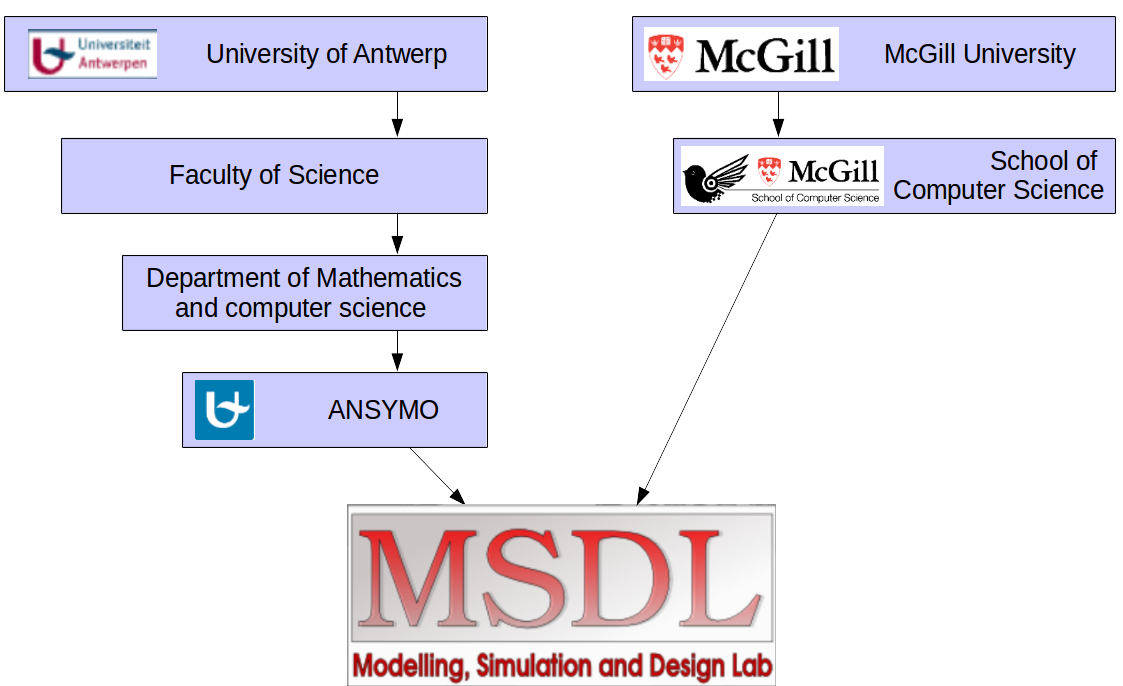
\includegraphics[width=0.8\linewidth]{msdl_organisation}

  \caption{Position of MSDL}
  \label{fig:msdl_org}
\end{figure}

The MSDL laboratory have members in two school, most part of these members are in the University of Antwerp but there is also some PhD students in the McGill University. McGill University is an English-language public research university in Montreal, Canada. You can see on the figure \ref{fig:msdl_org} a description of the organization of these universities\footnote{Only departments which belongs msdl were presented} and the position of MSDL in this organization.


\section{Description of MSDL}


\begin{figure}[!h]
  \centering
  
\includegraphics[width=0.6\textwidth]{MSDLbanner}
  \caption{MSDL banner}
  \label{fig:msdl}
\end{figure}


\begin{quotation}
<<The Modelling, Simulation and Design lab (MSDL) headed by Prof. Hans Vangheluwe is part of the School of Computer Science of McGill University in Montreal, Quebec, Canada and of the AnSyMo (Antwerp Systems and software Modelling) group in the department of Mathematics and Computer Science of the University of Antwerp, Antwerp, Belgium. The MSDL has projects, researchers and students in both locations.>>\cite{msdl}
\end{quotation}


So MSDL is a laboratory of Modeling. It is an important field of computer science because that could permit to create an engineering language understandable by everybody because it is based on graphical diagram. That also permit to create software without programming, just with logical diagram. I had the opportunity during my internship to participated in a presentation of all research subject. The figure \ref{fig:subject} is a not exhaustive list of all research topics discussed in MSDL. The part the most in connection with my subject was \textit{Simulation} and \textit{Analysis, Validation, Verification, Testing, and Accreditation} for obvious reasons.


\begin{figure}[h]
  \centering
  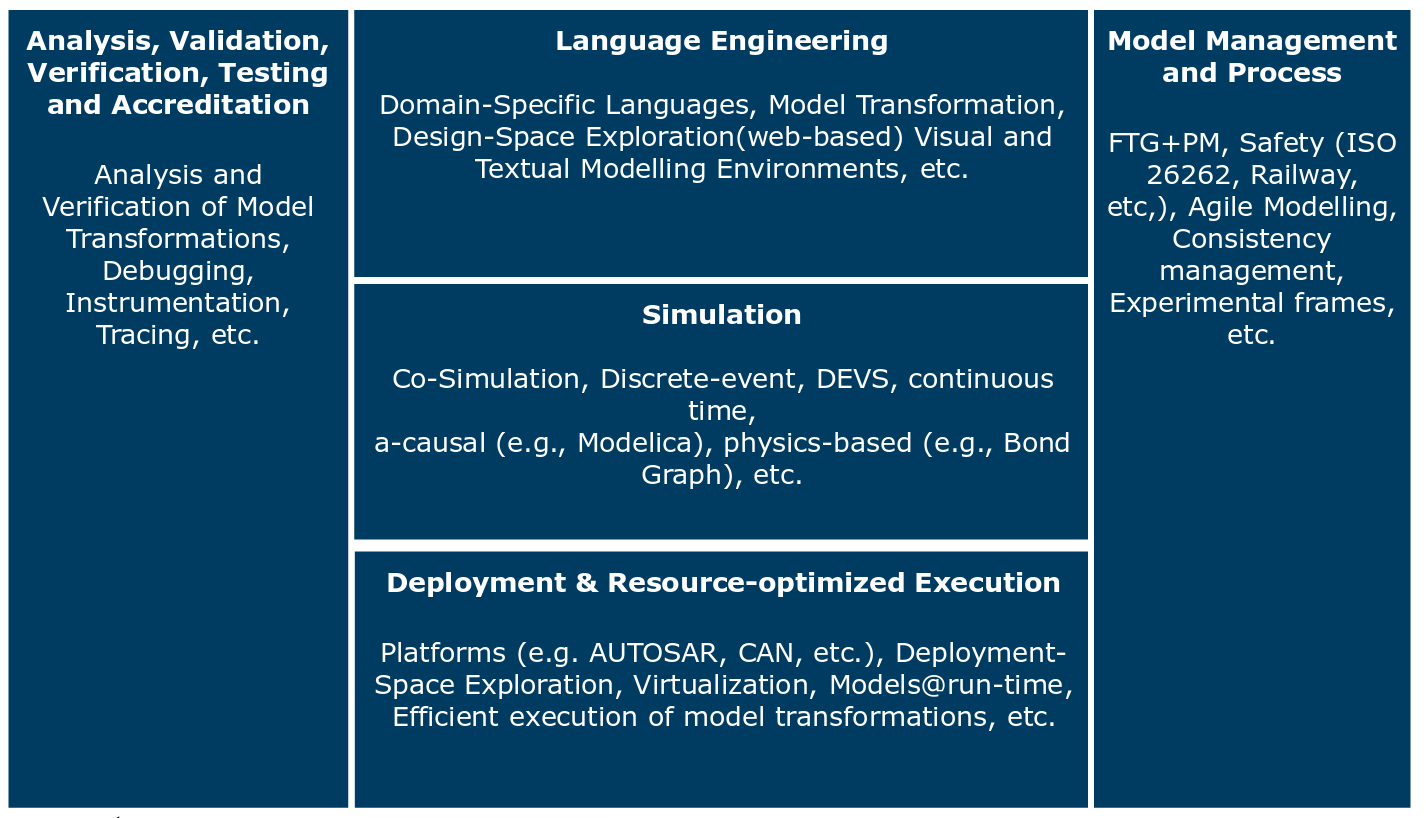
\includegraphics[width=\linewidth]{research}
  \caption{Research topics}
  \label{fig:subject}
\end{figure}



%%% Local Variables:
%%% mode: latex
%%% TeX-master: "../rapport_de_base"
%%% End:

\chapter{\umld}
\label{chap:UMLDesigner}


\umld is an open-source tool to edit and visualize UML2 models created by the French company:
\textit{Obeo}. The project is licensed under the EPL\footnote{Eclipse public license}

\begin{figure}[h] \centering
  
\includegraphics[width=0.3\textwidth]{logo}
  \caption{UML Designer logo}
  \label{fig:logo}
\end{figure}

\section{Utilization}

\umld is a graphical modeling tool for UML2 as defined by OMG\footnote{Object Management Group\cite{omg}}. As
you can see on the figure \ref{fig:umldesigner}, it permit to create diagram on which ones it is
possible to add some elements. The type of the elements proposed depend on the types of the diagram
chosen. For example, if you choose a \textit{User case diagram} it is possible to add 'user'
component that is impossible in \textit{Class diagram}.

So with graphical action it is possible to create many UML diagram which have transverse elements.

To finish, it is possible to create the code of the application that you have develop from the
model.


\begin{figure}[h] \centering
  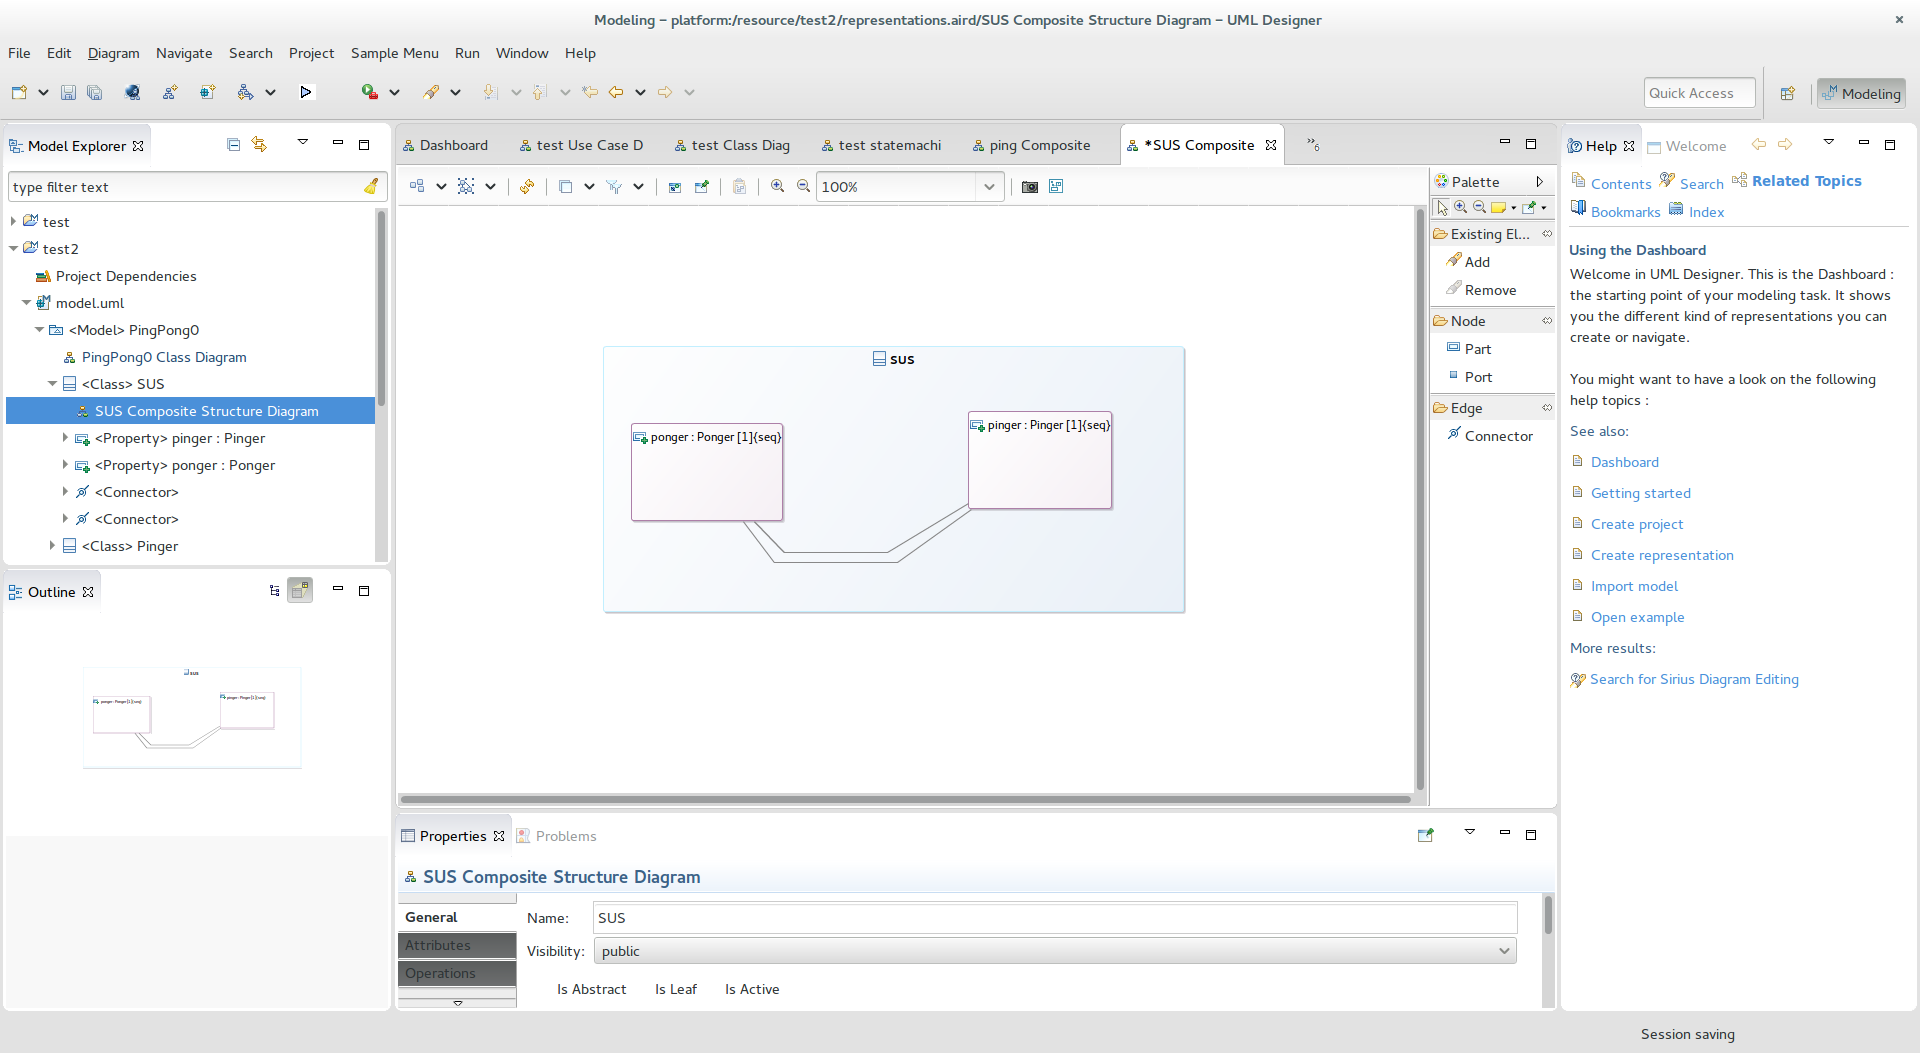
\includegraphics[width=0.8\textwidth]{umldesigner}
  \caption{Screen shot of \umld}
  \label{fig:umldesigner}
\end{figure}



\section{List of diagram supported}

\begin{itemize}
\item Packages diagram
\item Use case diagram
\item Activity diagram
\item Class diagram
\item Component diagram
\item Composite Structure diagram
\item Sequence diagram
\item State Machine diagram
\item Documentation table
\item Use Case cross table
\item Package containment diagram
\item Profile diagram
\end{itemize}



\section{Released}
\begin{center}

  \begin{tabular}{|c|c|}
    \hline
    \textbf{Version} & \textbf{Release Date} \\
    \hline
    1.0.0 &2012\\
    \hline
    2.0.0 &17 January 2013\\
    \hline
    2.1.0 &1 February 2013\\
    \hline
    2.2.0 &12 April 2013\\
    \hline
    2.3.0 &13 June 2013\\
    \hline
    2.4.0 &13 September 2013\\
    \hline
    3.0.0 &17 January 2014\\
    \hline
    4.0.0 &8 July 2014\\
    \hline
    4.0.1 &5 August 2014\\
    \hline
    5.0.0 &29 May 2015\\
    \hline
    \cellcolor{green}6.0.0 &19 October 2015\\
    \hline
  \end{tabular}

  \begin{tabular}{c}
    Legend:\\
    \cellcolor{green}Latest stable release\\
  \end{tabular}

\end{center}

\section{Base on}

\umld is based on a Eclipse and Sirius. It is a UML2 Eclipse plugin.

\subsection{Sirius}
Sirius is an open-source software project of the Eclipse Foundation. Sirius allows to create graphical modeling workbench. It include EMF\footnote{Eclipse Modeling Framework} and GMF\footnote{Graphical Modeling Framework}. On the figure \ref{fig:sirius}, it is possible to see the architecture of Sirius.


\begin{figure}[h]
  \centering
  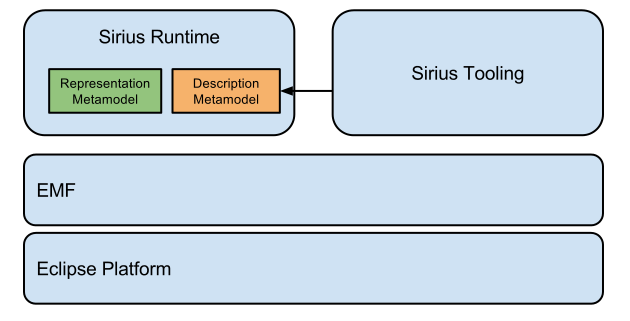
\includegraphics[width=\textwidth]{sirius_archi}
  \caption{Sirius architecture\cite{sirius}}
  \label{fig:sirius}
\end{figure}

\subsection{Eclipse}

\umld is base on Eclipse. 
The interface is the same as Eclipse. You can notice on figure
\ref{fig:umldesigner} that the menu are the same in the both software.



\begin{figure}[h] \centering
  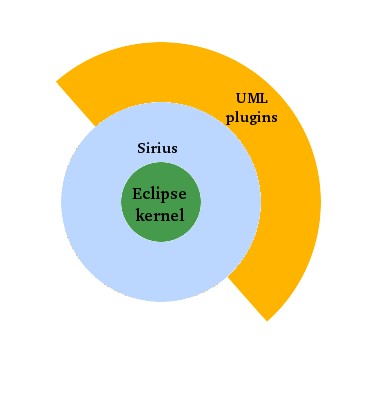
\includegraphics[width=0.5\textwidth]{archi}
  \caption{The \umld kernel}
  \label{fig:kernel}
\end{figure}






%%% Local Variables:
%%% mode: latex
%%% TeX-master: "../rapport_de_base"
%%% End:


\chapter{Simulator}

\section{Description}


At the beginning of this project, we had at our disposal the simulator of Mr Teodorov (figure \ref{fig:sim}). This simulator have a graphic user interface as you can see on the figure \ref{fig:sim}.


\begin{figure}[h]
  \centering
  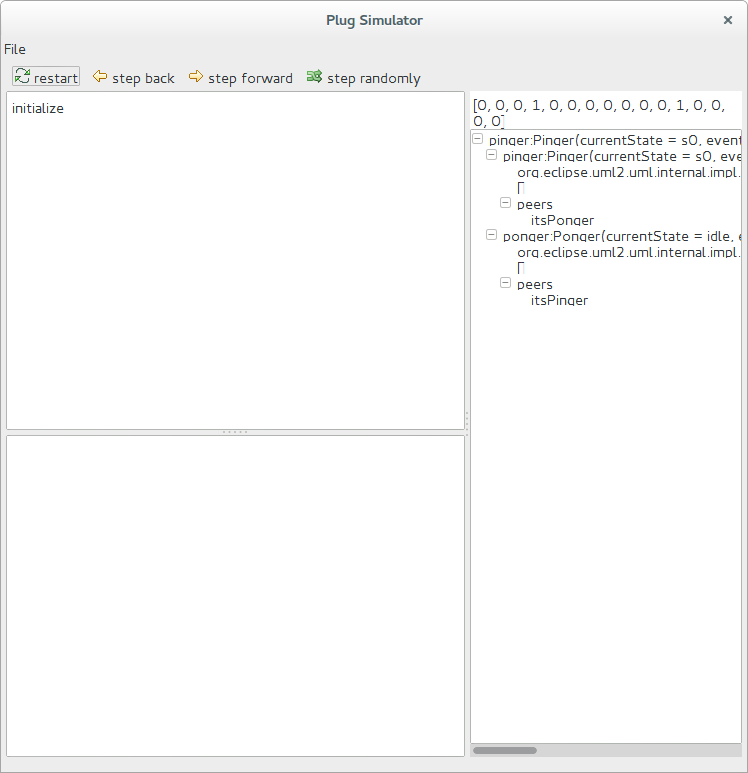
\includegraphics[width=0.5\textwidth]{simulator}
  \caption{Mr Teodorov simulator}
  \label{fig:sim}
\end{figure}


The simulator is compose on 4 part.
\begin{itemize}
\item On the top: some buttons to select an action
\item On the top-left-corner: The list of the next step
\item On the bottom-left-corner: The State Machine associated to the Current State.
\item On the right: A visualization of the Statechart
\end{itemize}

\section{Specificity of the uml file}

This simulator simulate a uml file. The uml file need to have a particular architecture.

\umld to save the uml project use 2 files. The first is named ``model.uml'' and the second is named ``representation.aird''.

To work, the simulator need the \textit{model.uml} file. Moreover, this file need to contain some specifics feature. It need a class \textbf{SUS} which contain the declaration of all other classes and all other classes need to have a State Machine diagram associated. You can see on the figure \ref{fig:simulateur}, that all classes need to have their own State Machine diagrams.

\begin{figure}[h!]
  \centering
  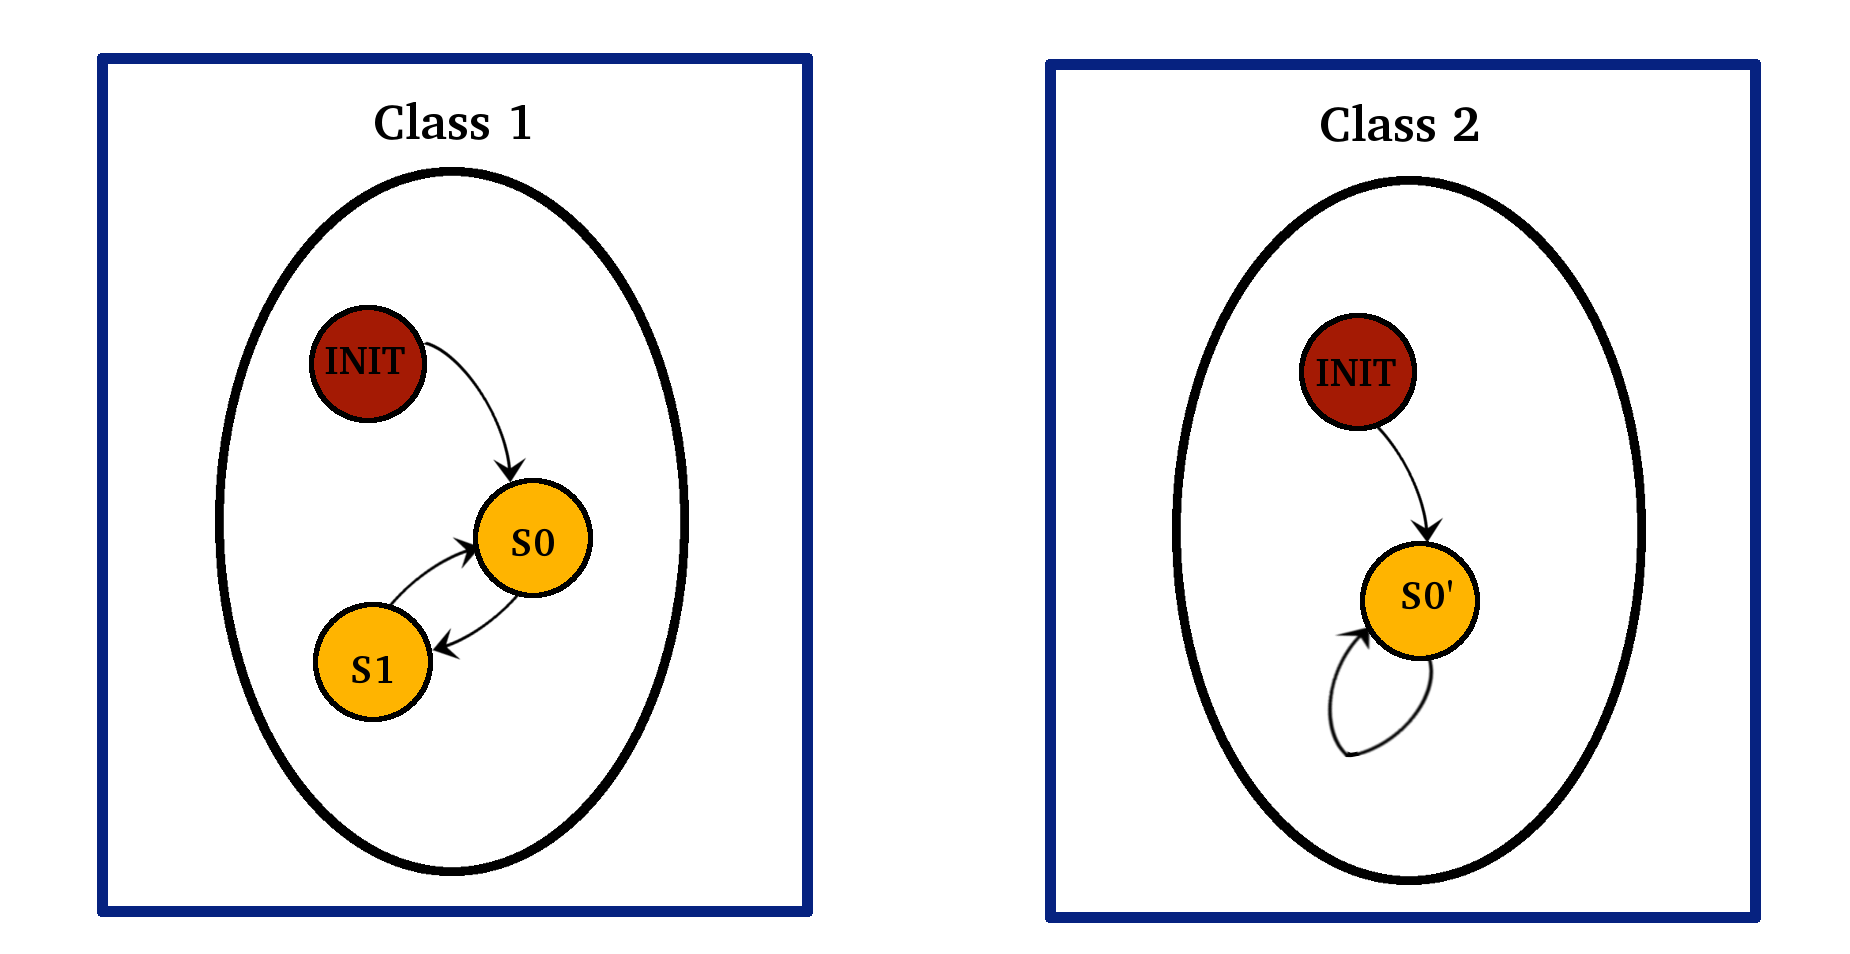
\includegraphics[width=\textwidth]{simulation}
  \caption{representation of the most important elements of the simulator}
  \label{fig:simulateur}
\end{figure}




%%% Local Variables:
%%% mode: latex
%%% TeX-master: "../rapport_de_base"
%%% End:


\part{Study of the subject}


\chapter{Communication inter process}

\section{Type of communication conceivable}

A lot of type of communication inter process were suggested to create a discussion enter the plugin and the simulator. But we will present only the most consistent.

The communication is the part the most important of this project, because that will implement the interface between the two software.

\subsection{Socket}

\begin{tabular}{|p{0.45\textwidth}||p{0.45\textwidth}|}
\hline
  \textbf{Advantages}&\textbf{Drawback}\\
\hline
Work with every simulator type (python, java, ...) & communication synchronous\\
\hline
\end{tabular}

\subsection{File}

\begin{tabular}{|p{0.45\textwidth}||p{0.45\textwidth}|}
\hline
  \textbf{Advantages}&\textbf{Drawback}\\
\hline
Problem when two software want to change the same file at the same moment& Communication asynchronous\\
\hline
\end{tabular}

\subsection{Named pipe}

\begin{tabular}{|p{0.45\textwidth}||p{0.45\textwidth}|}
\hline
  \textbf{Advantages}&\textbf{Drawback}\\
\hline
It is possible to use the Simulator outside the graphical modeling tool & \\
\hline
\end{tabular}


\subsection{Shared Memory}

\begin{tabular}{|p{0.45\textwidth}||p{0.45\textwidth}|}
\hline
  \textbf{Advantages}&\textbf{Drawback}\\
\hline
It is possible to use the Simulator outside the graphical modeling tool & \\
\hline
\end{tabular}


\subsection{Thread}

\begin{tabular}{|p{0.45\textwidth}||p{0.45\textwidth}|}
\hline
  \textbf{Advantages}&\textbf{Drawback}\\
\hline
&Need to recode the simulator \\
\hline
\end{tabular}


\subsection{Our solution}

The solution was not in this list of common way to communicate inter process. In fact, we use the \textit{Runtime} class which is in the java library.~\\


\begin{tabular}{|p{0.45\textwidth}||p{0.45\textwidth}|}
\hline
  \textbf{Advantages}&\textbf{Drawback}\\
\hline
It is possible to use the Simulator outside the graphical modeling tool & \\
\hline
Work with every type of simulator& \\
\hline
\end{tabular}





%%% Local Variables: 
%%% mode: latex
%%% TeX-master: "../rapport_de_base"
%%% End: 




%%%% CONCLUSION %%%%%%%%%

\chapter*{Conclusion}
\addcontentsline{toc}{chapter}{Conclusion}
\newpage

%%%% ANNEXE %%%%%%%%%%%%

\part*{Annexe}
\addcontentsline{toc}{part}{Annexe}
\appendix

\chapter{Organisation of the work}





%%% Local Variables: 
%%% mode: latex
%%% TeX-master: "../rapport_de_base"
%%% End: 



\nocite{*}
%\input{annexe_}
\newpage
~\\
\newpage
 \listoffigures
 \printindex
 \bibliographystyle{plain}
  \bibliography{biblio}

\end{document}
%%%%%%%%%%%%%%%%% FIN DU DOCUMENT
%%% Local Variables:
%%% mode: latex
%%% TeX-master: t
%%% End:
